
\section{Similar solutions}

	\subsection{Parallel Kingdom - Age of Ascension}
	This game was on market for 8 years (2008-2016). Parallel Kingdom is a closest solution to ours.
	
	
	”Parallel Kingdom is a mobile, location based, massively multiplayer game that uses GPS
	location and Google Maps to place users in a virtual world. Parallel Kingdom is the first
	location based RPG for the iOS and Android platforms. The game is set in a virtual world
	or ”Parallel Kingdom” where users claim their territories based on their GPS location or by making friends who invite them to travel to new places. Parallel Kingdom is a freemium
	game and utilizes a virtual goods revenue model.”
	
	\subsection{Ingress}
	Developed by Niantic, which was then part of Google, this game was released in 2013 for
	Android and in 2014 for iOS.[4] It is a location based, massively multiplayer game. A player have to choose one of the two factions, Enlightened or Resistance, and then as a part of his 	team capture regions of the game map. A faith of each faction relies on players’ cooperation. Thanks to that players meet in real life and coordinate their actions.
	
	Ingress was the first very successful augmented reality game with more than 10 000 000
	installs.
	
	\subsection{Pokémon GO}
	After its success with Ingress, Niantic started working on a new game Pokemon GO. Once
	released, the game became incredible hit. Even though the game faced many problems during
	its launch, mainly caused by the unexpected success and more active users than Pokémon
	GO was able to handle, in the first 80 days Pokémon GO reached about 550 millions downloads and earned about \$470 million.
		
	The game is very similar to Ingress and uses the same crowd-sourced geographical data.
	
\section{Use Cases}
	\subsection{Actors}
		\begin{figure}[h]	
			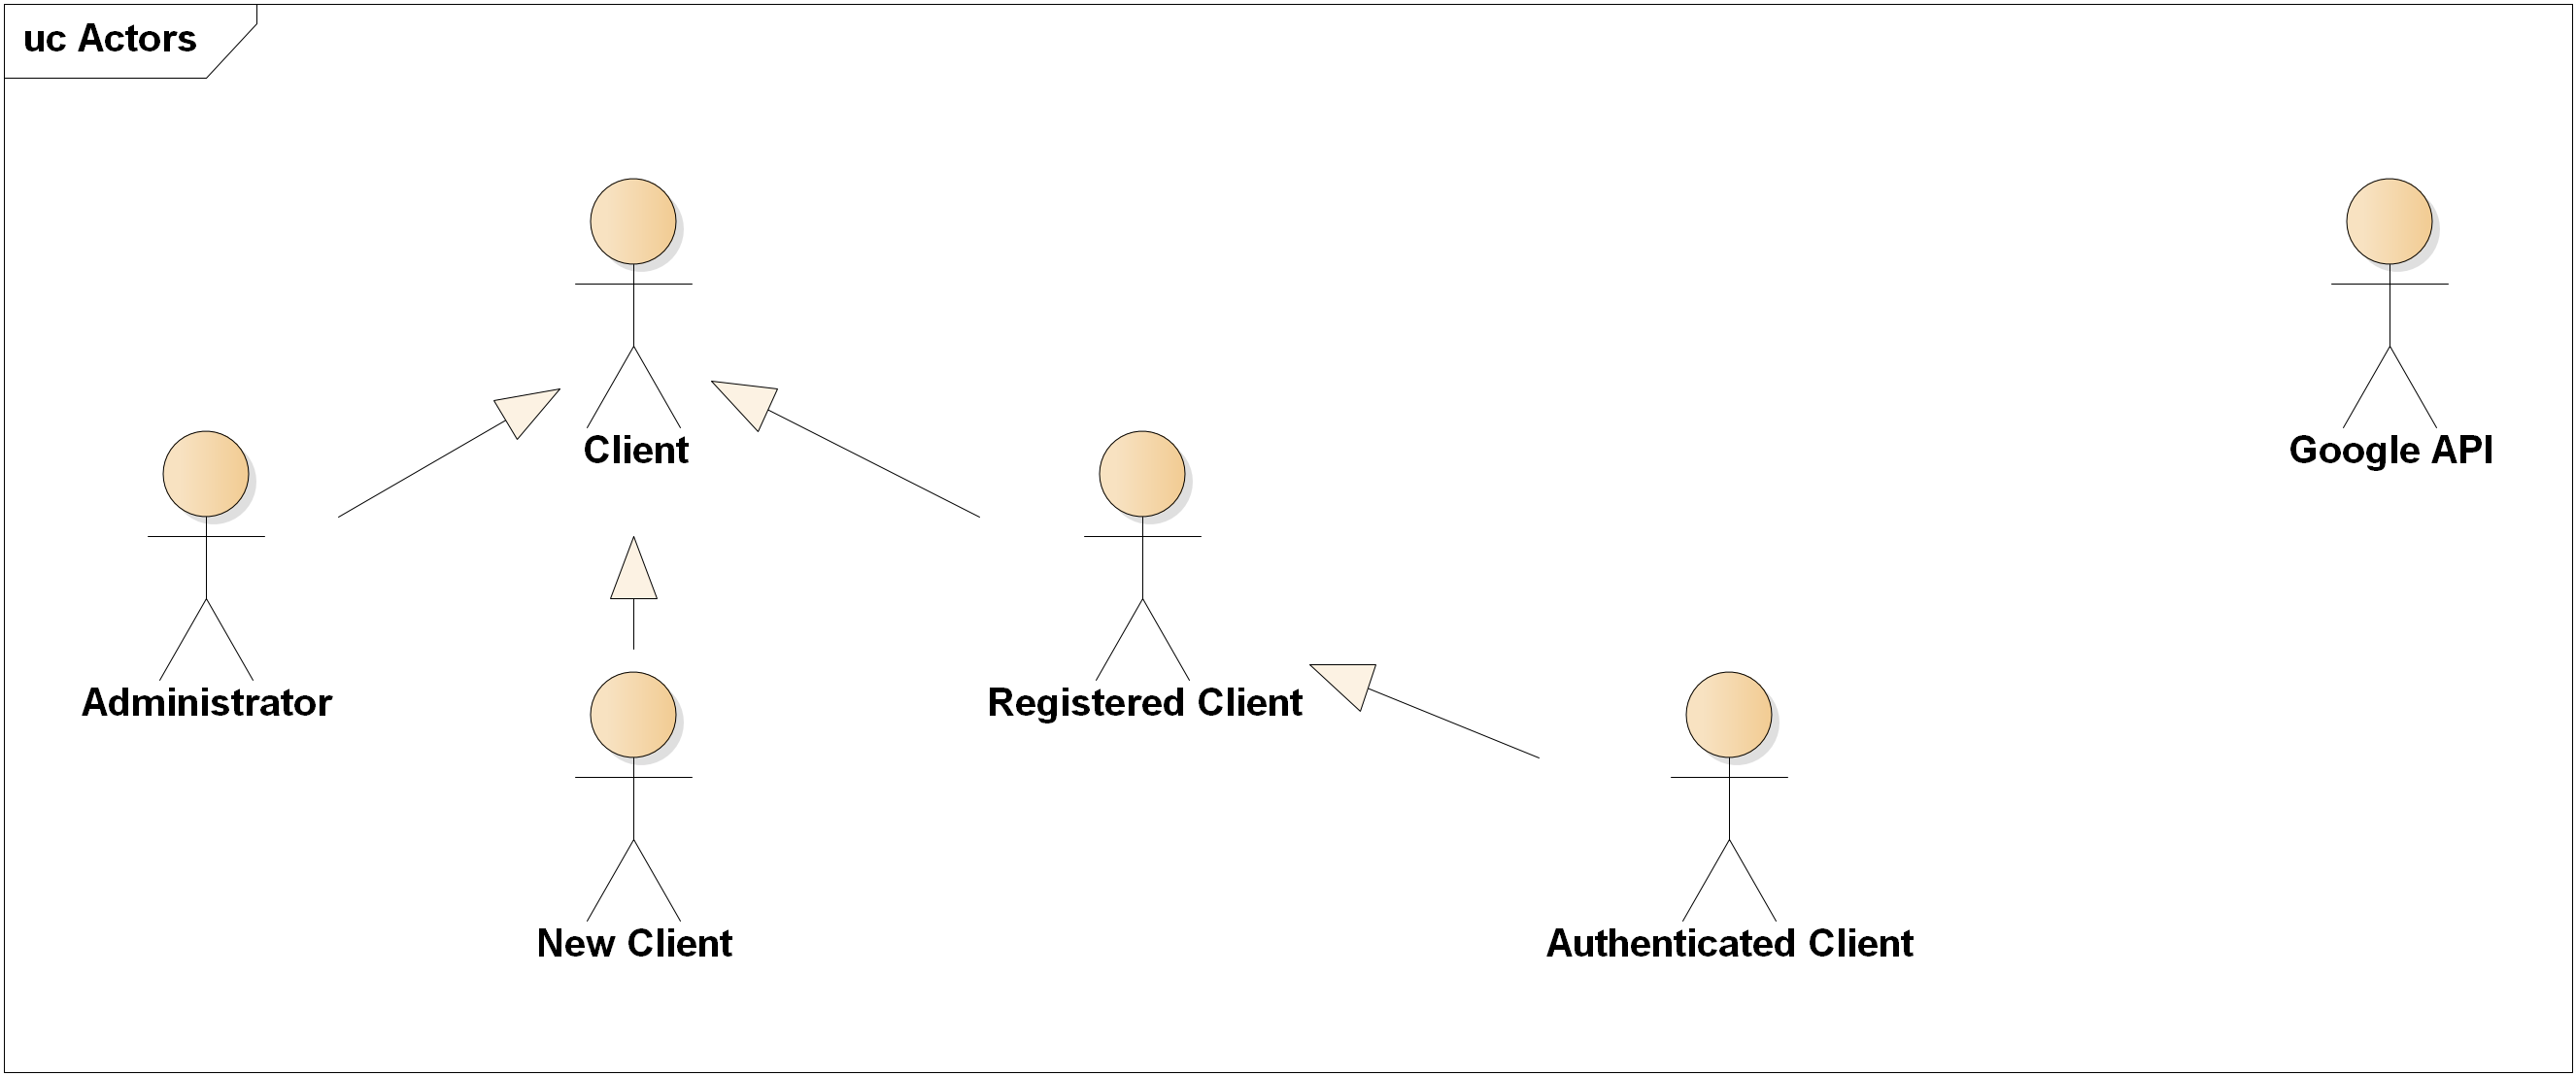
\includegraphics[width=\textwidth]{figures/UC_Actors}
			\centering			
			\caption{Use Cases Diagram -- Actors}
			\label{fig:ucactors}
		\end{figure}
		\noindent Actor is a role played by a user or other system that interacts with the server. The most general role is \textit{Client} and anyone who accesses the server through API is considered to play either this role or any of its children. From now on, the terms client and user will be used interchangeably. Refer to Figure \ref{fig:ucactors} for the role hierarchy.
		
		\textit{Administrator} is a client who has privilege to create and maintain the functionality of the server. \textit{New Client} is a user who is not yet registered and probably accesses the game for the first time. \textit{Registered Client} is the default role for a user who already has a valid account but is not logged in. Lastly, \textit{Authenticated Client} has all the required privileges to play the game. This client will be refereed to as \textit{player}. The last main actor is Google API which provides the access to Google services. 		
	
	\subsection{Actions}	
		\begin{figure}[h]	
			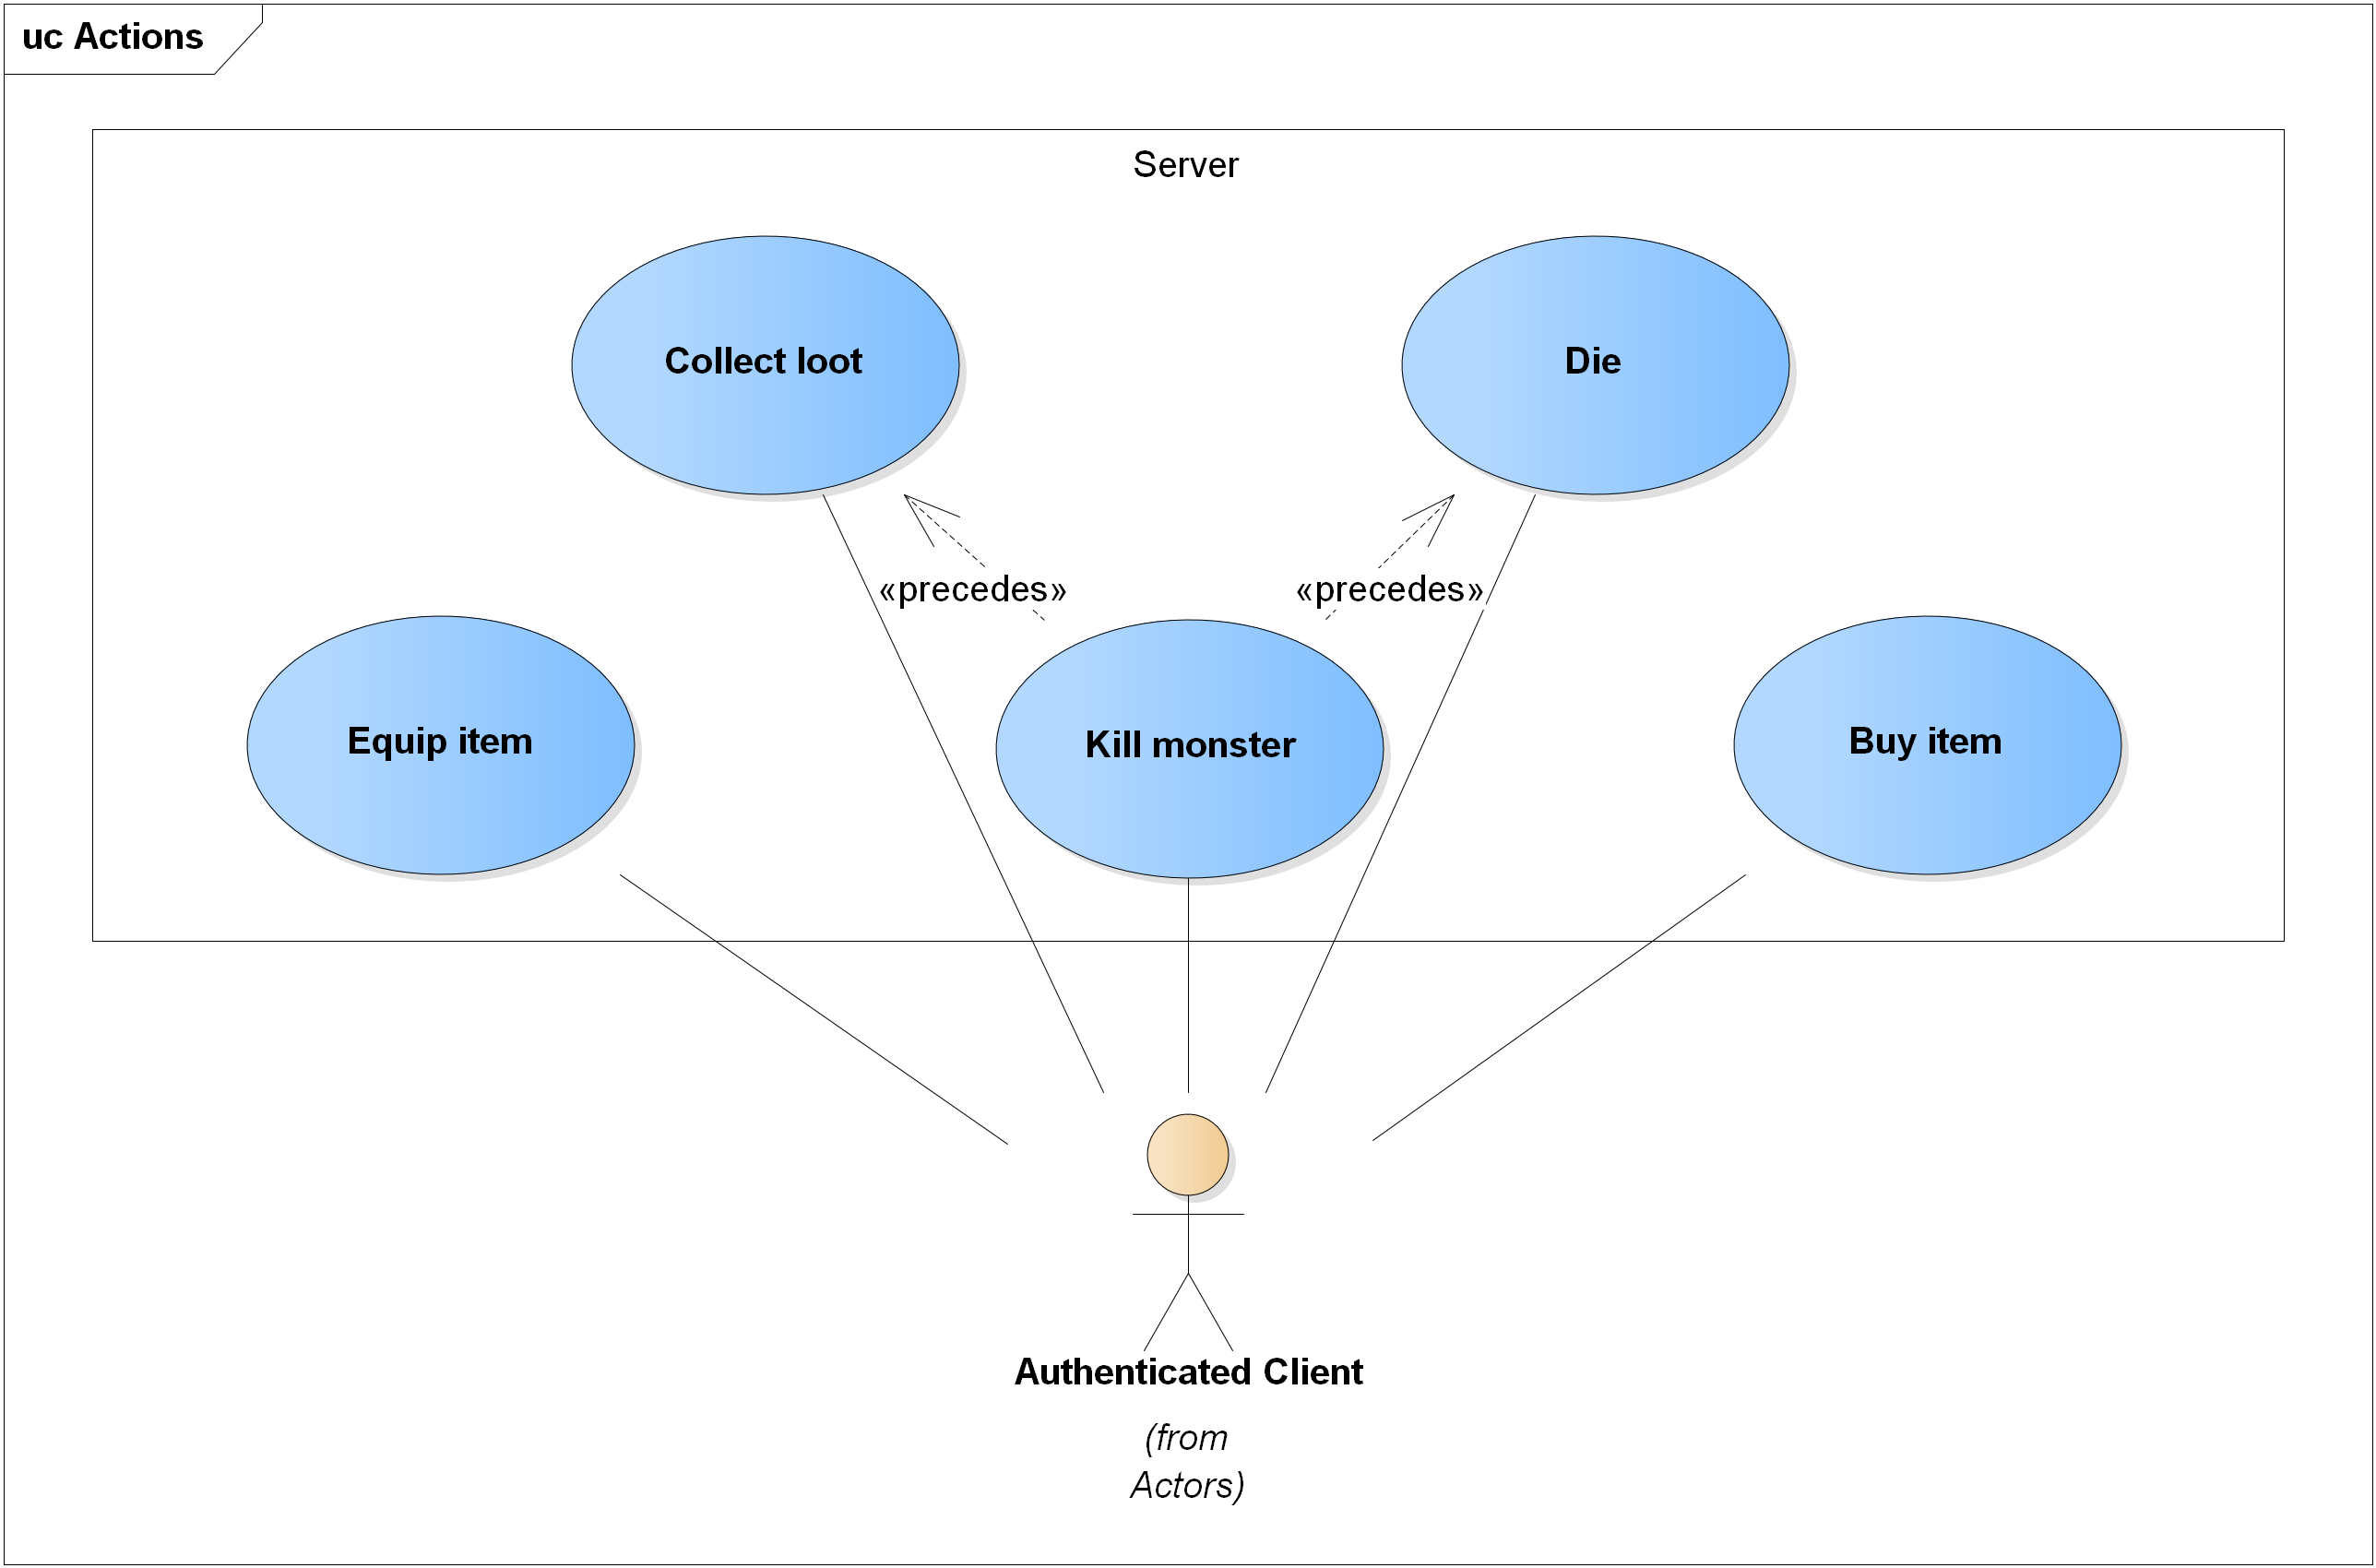
\includegraphics[width=\textwidth]{figures/UC_Actions}
			\centering			
			\caption{Use Cases Diagram -- Player's actions}
			\label{fig:ucactions}
		\end{figure}
		\noindent Actions is an event triggered by player's interaction with a game object. See Figure \ref{fig:ucactions}.
		
		\begin{itemize}
			\item \textbf{Equip item} \\
			A player wants to equip an item from his inventory. The item will be assigned to a specific slot. For example the player equips a sword to his right hand.
			
			\item \textbf{Buy item} \\
			A player wants to exchange gold in a shop for an item he chooses. When the purchase is finished, the player receives the item to his inventory.
			
			\item \textbf{Kill monster} \\
			A player wants to kill monsters to progress in the game. If he successfully kills the monster, he is rewarded with gold and experience
			
			\item \textbf{Collect loot} \\
			This action must be preceded by the \textit{Kill monster} use case. A player can choose to collect loot from the monster he killed.
			
			\item \textbf{Die} \\
			This action must be preceded by the \textit{Kill monster} use case. A player who lost his fight against a monster dies and is punished with some penalty.		
		\end{itemize}

	\subsection{Authentication}
	\begin{figure}[h]	
		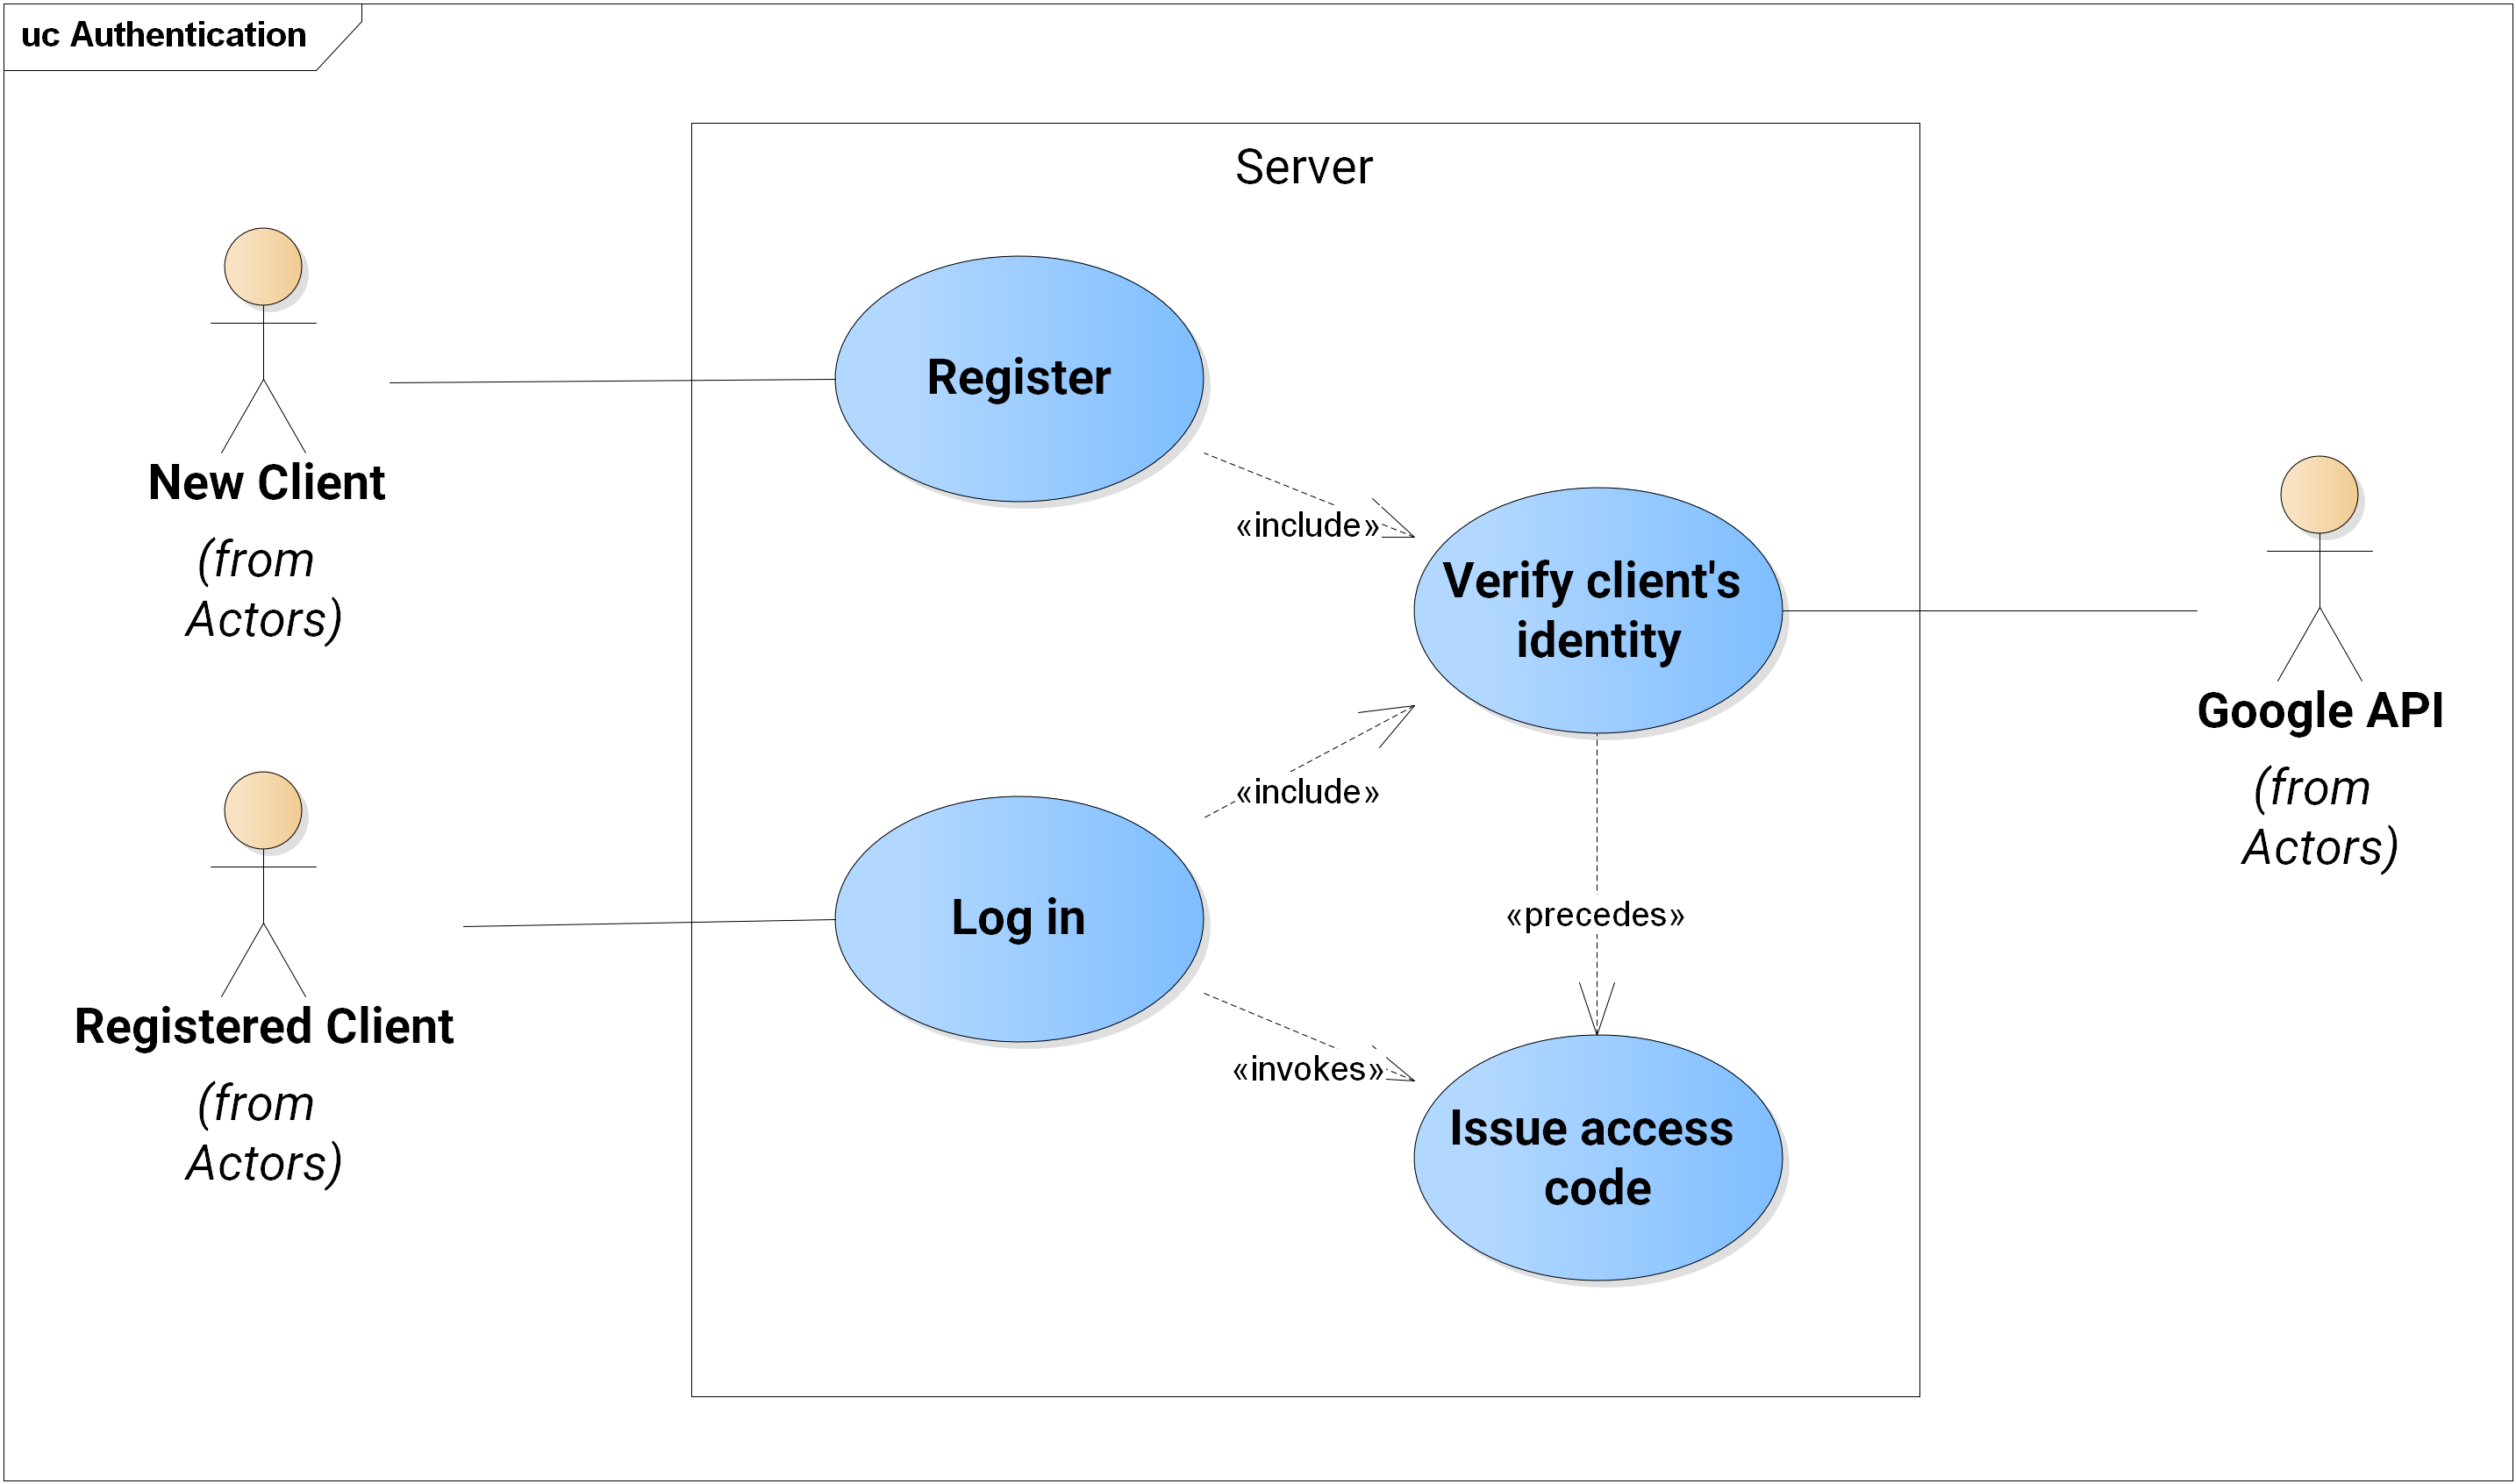
\includegraphics[width=\textwidth]{figures/UC_Authentication}
		\centering			
		\caption{Use Cases: Client's authentication}
		\label{fig:ucauth}
	\end{figure}

	\subsection{Miscellaneous}
	\begin{figure}[h]	
		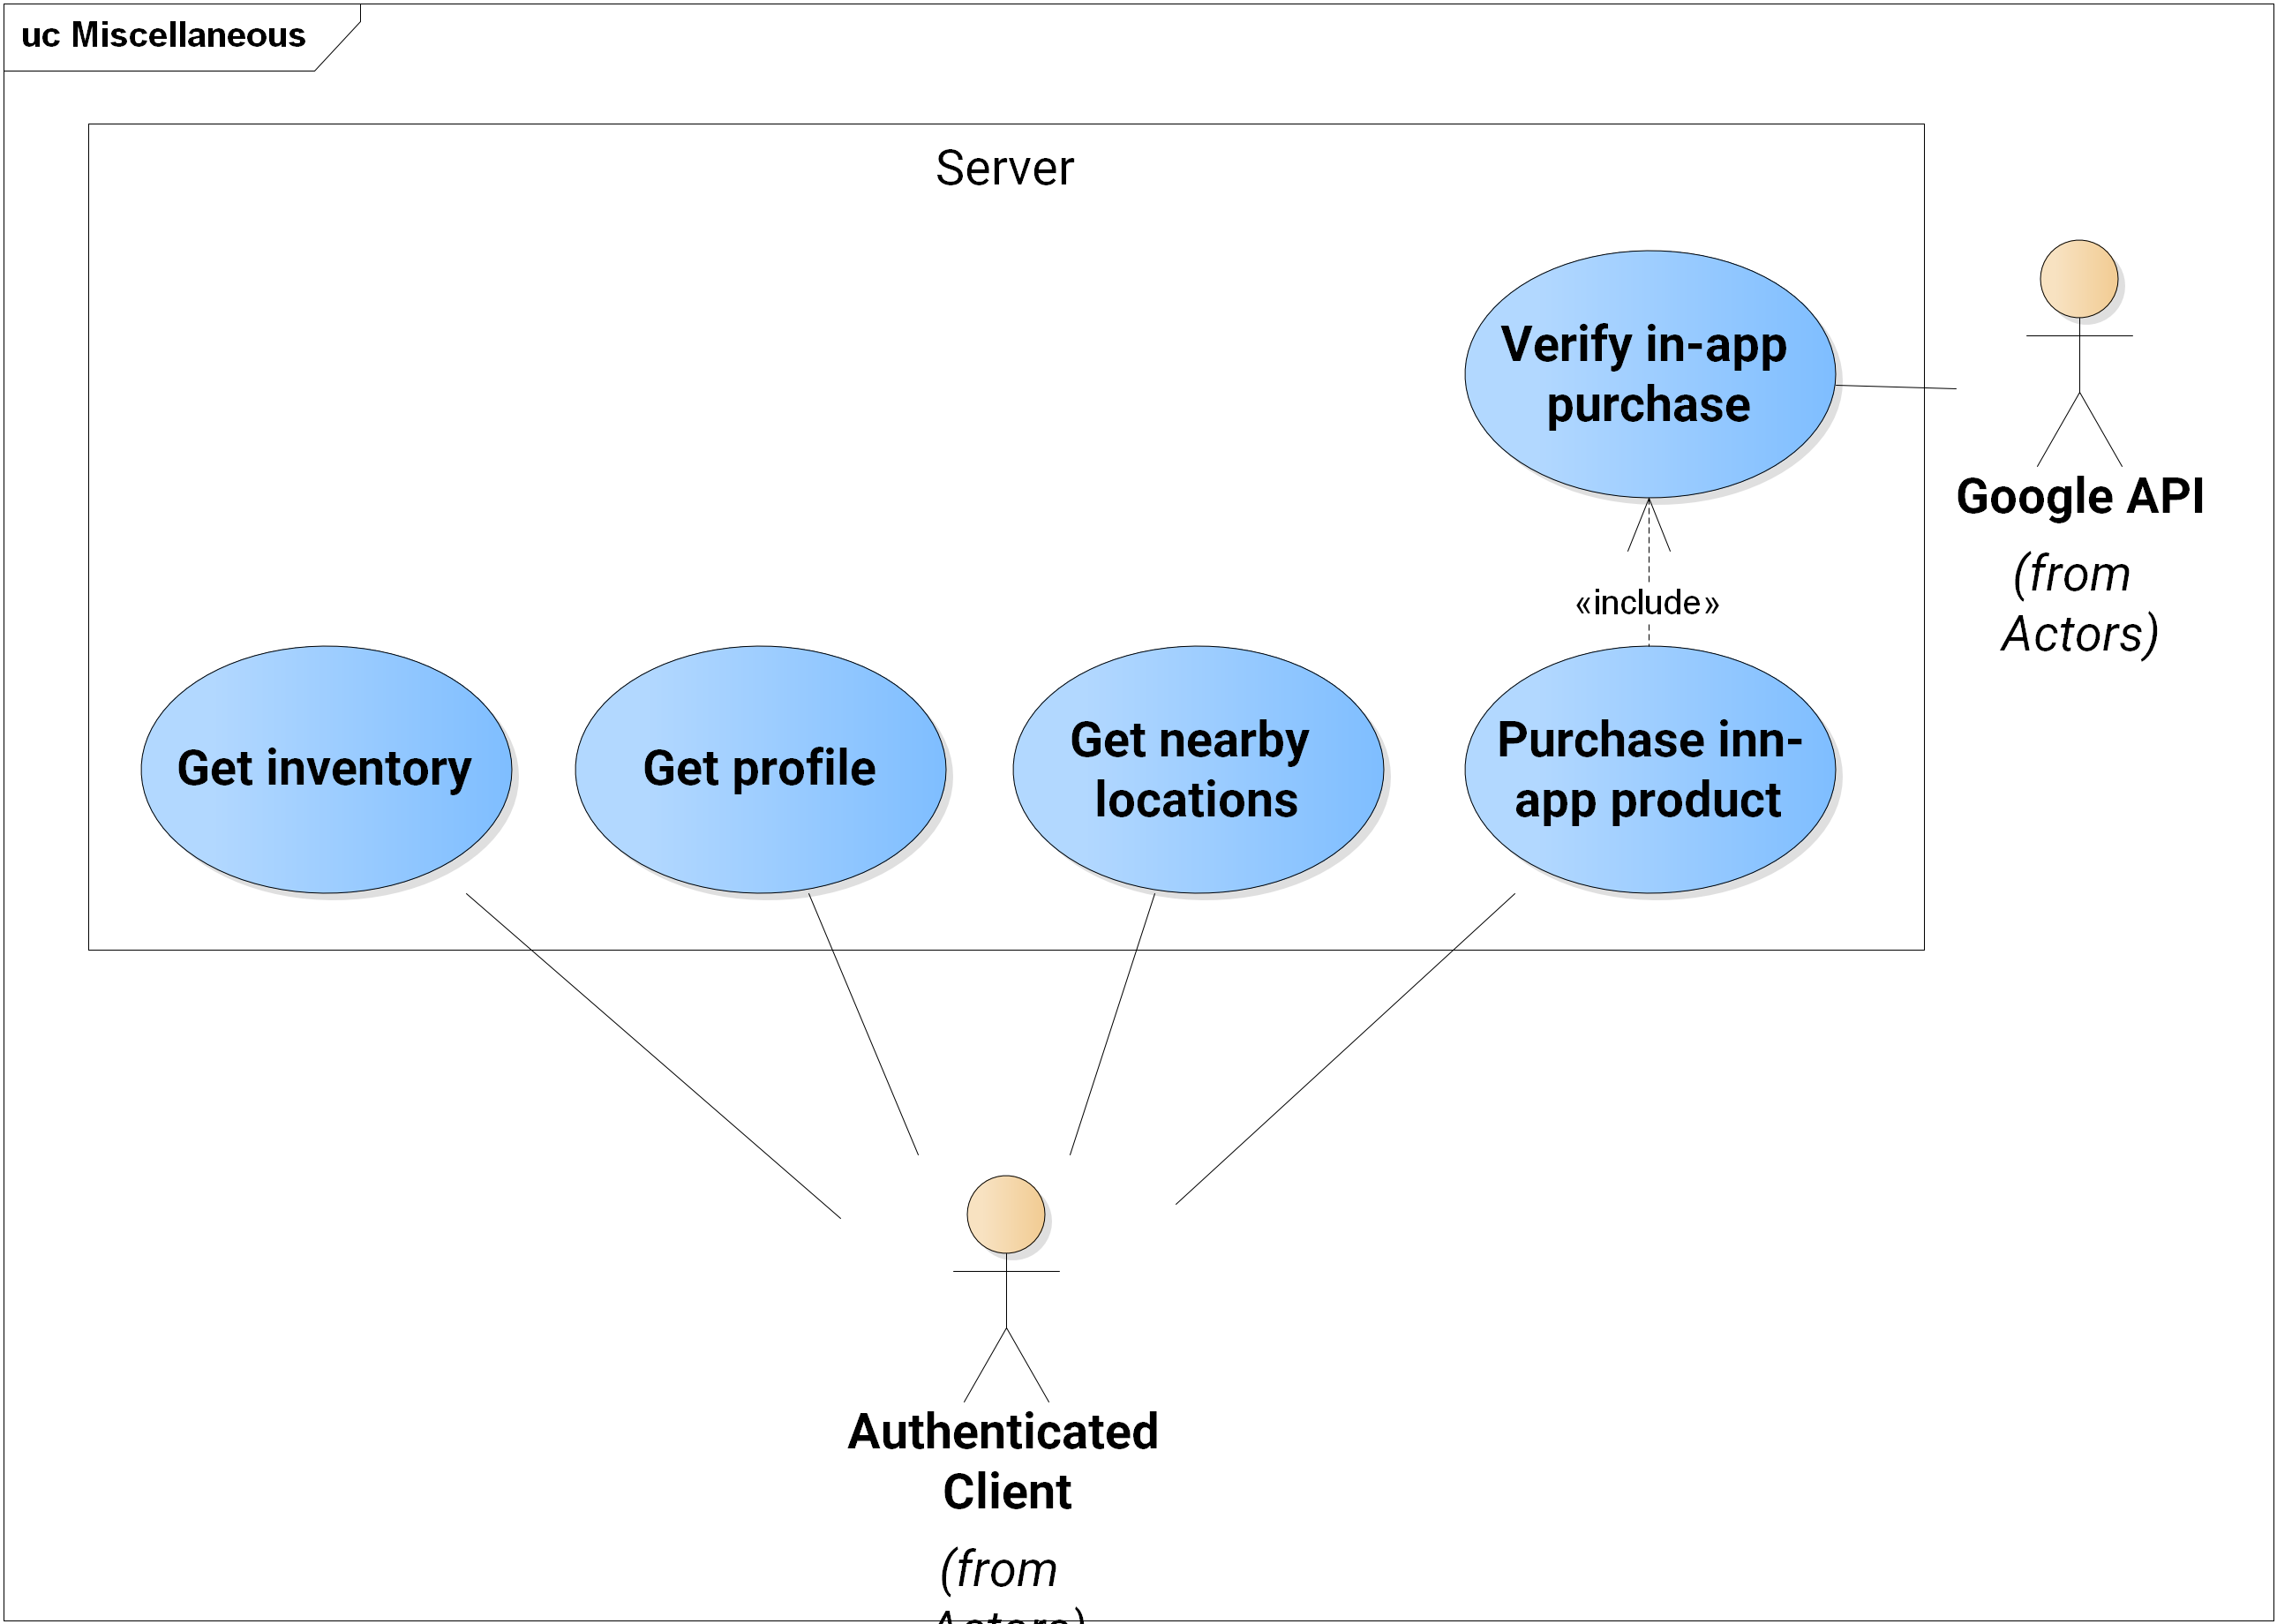
\includegraphics[width=\textwidth]{figures/UC_Miscellaneous}
		\centering			
		\caption{Use Cases: Miscellaneous}
		\label{fig:ucmisc}
	\end{figure}

	\subsection{Administration}
	\begin{figure}[h]	
		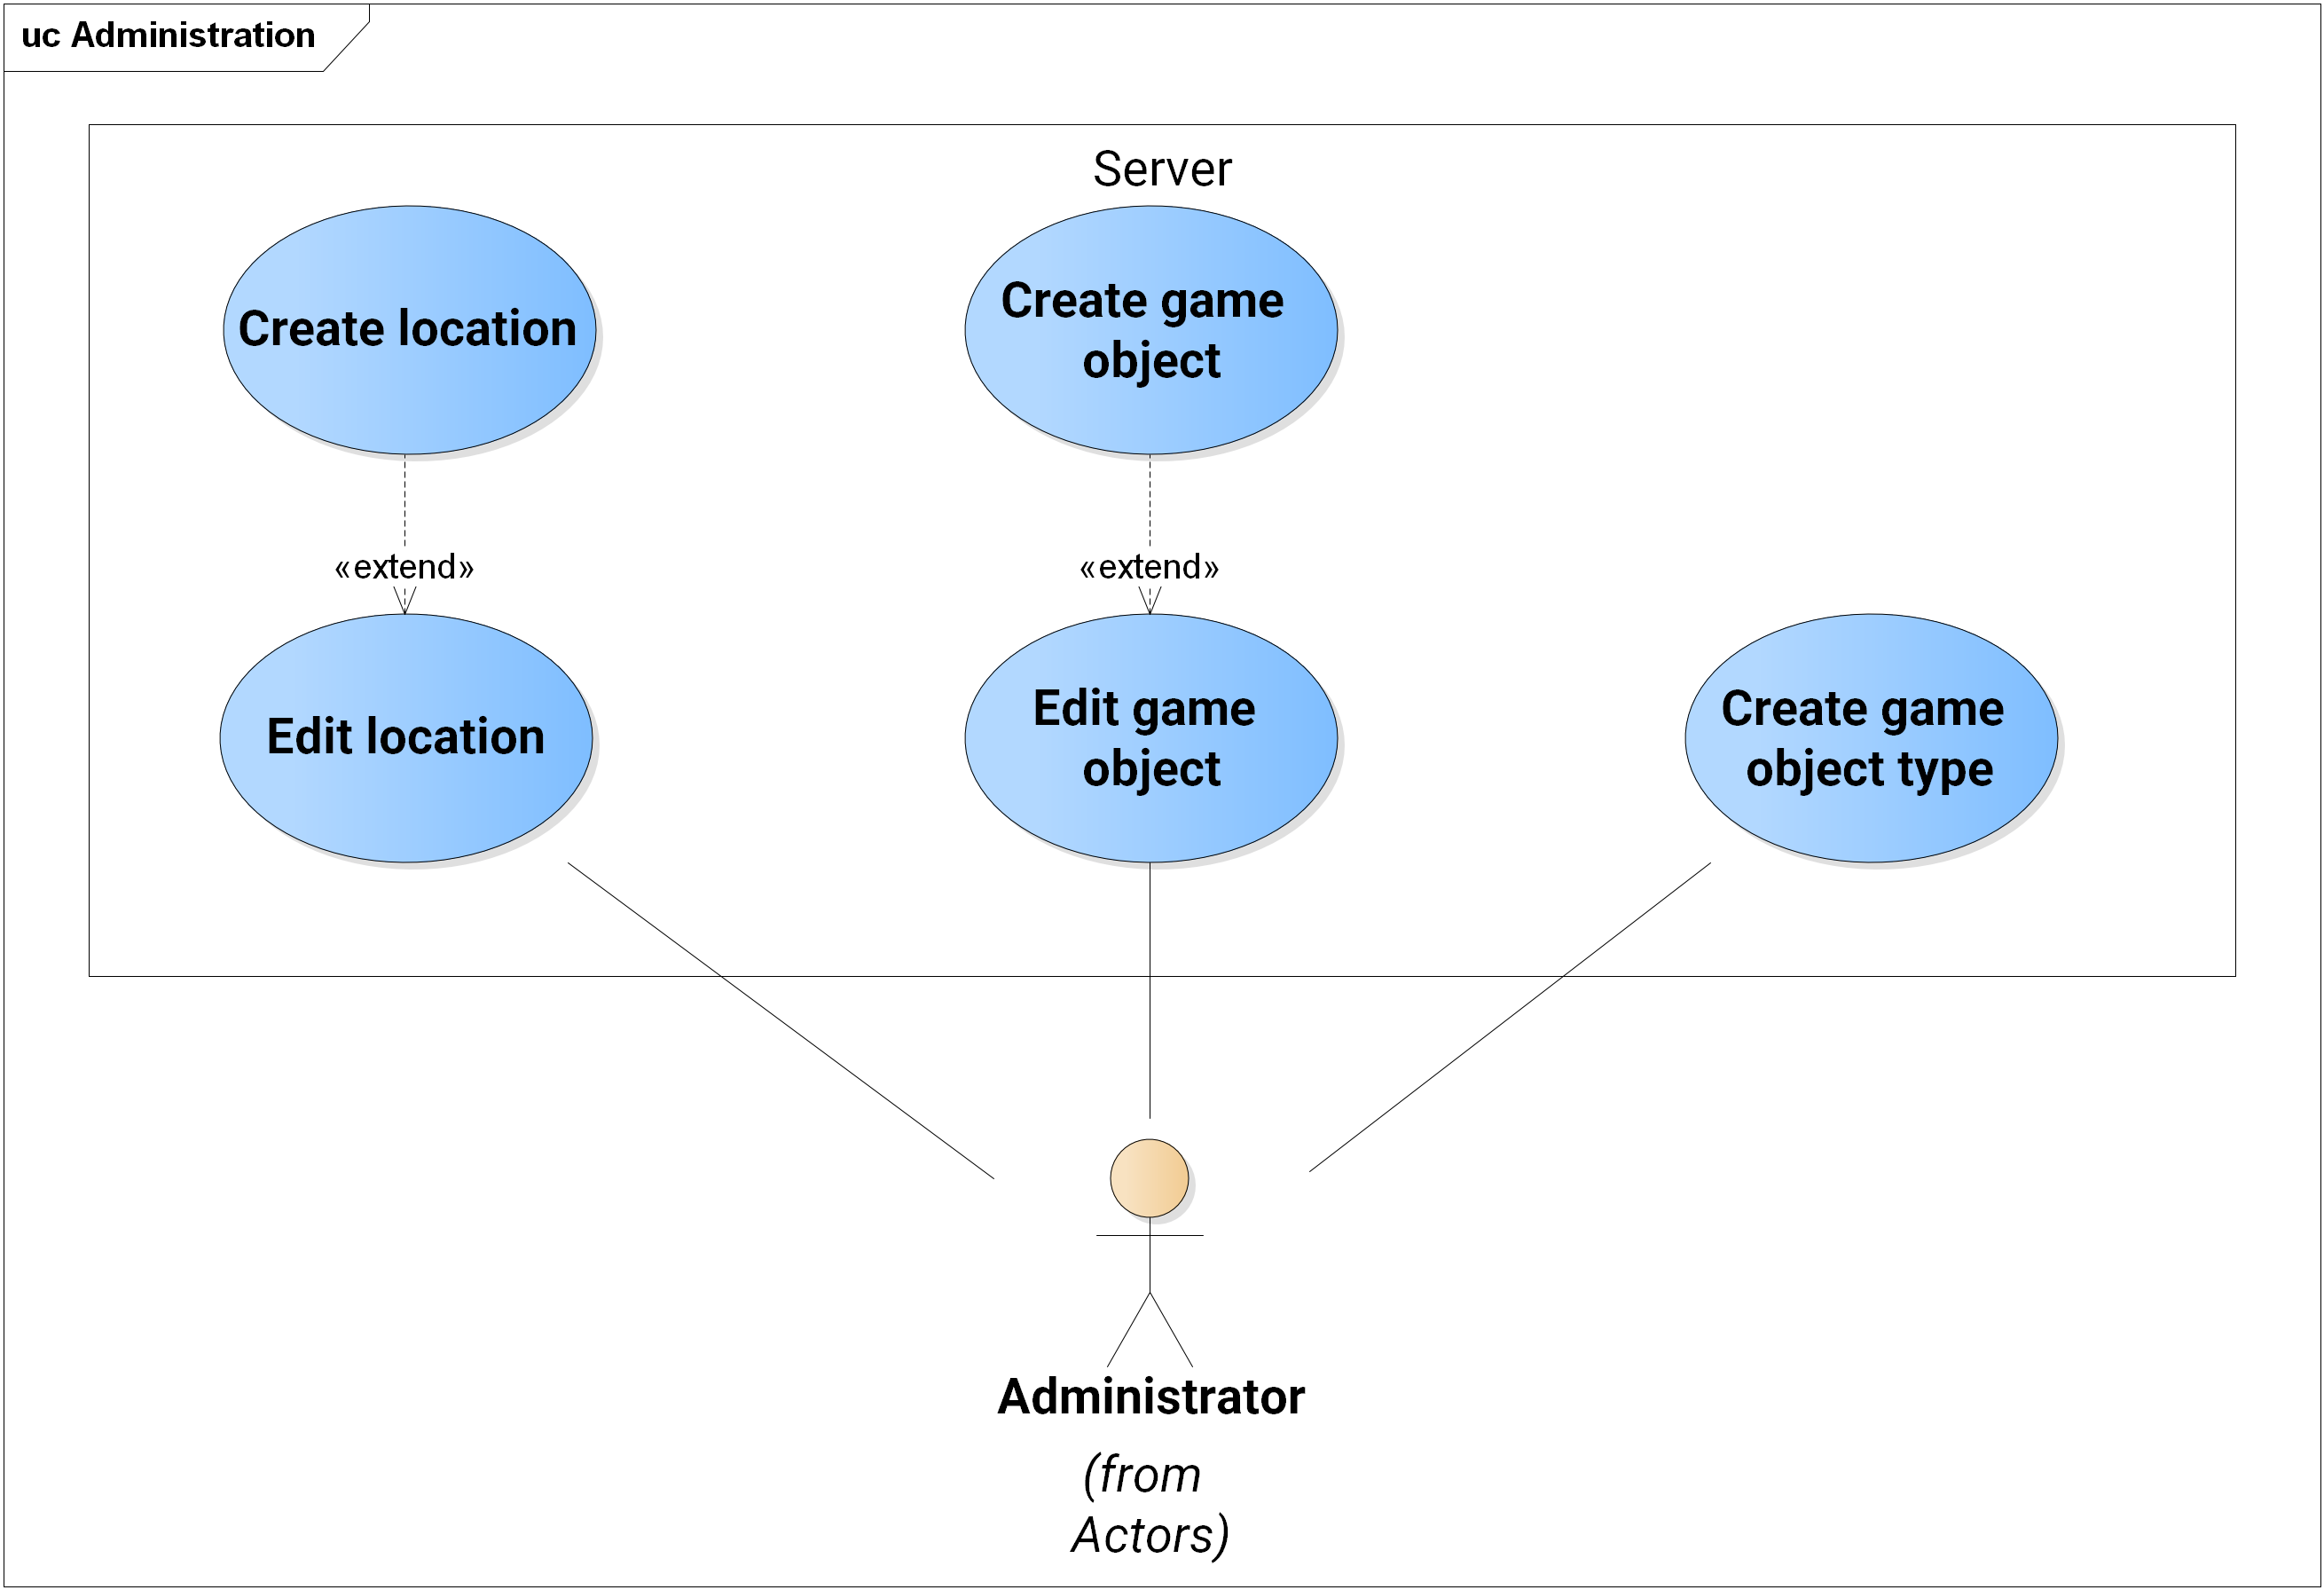
\includegraphics[width=\textwidth]{figures/UC_Administration}
		\centering			
		\caption{Use Cases: Administration}
		\label{fig:ucadmin}
	\end{figure}	
	
	
\section{Requirements}

	\subsection{Functional Requirements}
		\subsubsection*{Rules}
		\begin{enumerate}
			\item \textbf{The server must provide API to clients} \\
			The key requirement for the server is to allow receiving HTTP(S) requests. When processed, the server responds in JSON format.
						
			\item \textbf{The player's character has attributes} \\
			The character has a set of attributes, including health, experience, level, and owned gold. Maximum health increases with level. The experience is rewarded after certain actions, e.g. after killing a monster. The gold is primary in-game currency.
			  
			\item \textbf{A player can own items} \\
			A player has an inventory which can contain various types of items. The item can be for example sword, potion, armor etc.
			
			\item \textbf{A game object has a type and inherits all its properties} \\
			The type of game object specifies allowed actions, its attributes, default name and description.			
			
			\item \textbf{A game object can be a monster} \\
			The monster can be killed but can also inflict damage to the player. It has its own inventory and there's a reward for killing the monster in a form of gold and experience.
			
			\item \textbf{A game object can be a shop} \\
			The shop can contain several items with specified price.  
			
			\item \textbf{A game object can be an item} \\	
			The item can be one of the many objects useful to a player. Examples of the items are health potion, sword, armor, necklace and similar.
			
			\item \textbf{Each game object has its own inventory} \\
			The inventory contains other game objects. Example of this requirement is a monster with a potion and a sword in its inventory; both will be given to the player who kills the monster.  
			
			\item \textbf{The server stores a list of predefined locations} \\	
			Real geographic locations for the game objects are stored on the server to ensure every player has the same location-object pair. 
								
			\item \textbf{A game object can independently exist at many locations} \\
			This requirement aims to help maintain the game objects efficiently by administrators. It allows creating small set of abstract game objects with predefined inventories and other attributes. 
			
			\item \textbf{If a player kills a monster at a location, the monster will be hidden for a period} \\
			To prevent the player from killing the same monster continuously without a need of moving somewhere else, the location should be hidden for a certain period after the kill.
			
			\item \textbf{The server should provide API for administration} \\	
			Such API will be used to manage locations, create and edit game objects or to assign a game object to some locations. It is necessary to protect the administration endpoints from unauthorized access.
					
			\item \textbf{The server must persist player’s profile between sessions} \\
			All the player's attributes, his inventory and equipment must be stored between sessions. Player will continue from the state in which he ended.
			
		\end{enumerate}
		\subsubsection*{Features}
		\begin{enumerate}
			\item \textbf{A player registers and logs in the game using Google account} \\
			For the player's convenience, a Google account is required to play. The server does not have to store or handle any password. Most of the authentication process is delegated to Google servers.
			
			\item \textbf{A client can get nearby game objects based on his location} \\
			The major feature of this application is being location-aware. Server must provide a method to retrieve game locations near the requested latitude and longitude. The "near area" should be circular, defined by its radius; the size have to be carefully chosen so it's big enough to cover client's maps but also small to limit the response size and the spatial search overhead.
			
			\item \textbf{A player can kill a monster} \\
			When the player wins the fight, he will be rewarded by experience and gold. 			
			
			\item \textbf{A player can be killed be a monster} \\
			The player can lose health during the fight with a monster. If the health reaches zero, the player dies and loses an amount of gold based on his level.
			
			\item \textbf{A player can collect items from the monster he killed} \\
			When the player wins the fight, he's offered to collect items from the monster's inventory. He can chose any subset of these items.
			
			\item \textbf{A player can equip an item} \\	
			Many items in the game can be equipped. These items have predefined equipment slot, for example a sword have to be held in hand, an armor worn on chest, shoes put on feet and so on.
						
			\item \textbf{A player can buy object from a shop} \\
			Gold can be exchanged for various items in shops.
			
			\item \textbf{A player can use an item from his inventory} \\
			Some items in the game are consumables. When used, an action defined by the item is executed. For example a health potion heals the player.
			
			\item \textbf{A player can purchase in-app product} \\
			The application allow a user to exchange real-life currency for the in-game one. The server should verify such purchase and add the currency to his profile.
			
		\end{enumerate}
		
		
	\subsection{Non-functional}
	
		\begin{enumerate}
			\item \textbf{The data layer consists of a database engine and a caching} \\
			Game Server never accesses database directly. Data are retrieved from the database upon request and then cached. Upper layers communicate exclusively with cache.		
			
			\item \textbf{The server provides an API for client} \\
			The API support at least following:
			\begin{enumerate}
				\item Retrieve nearby game locations
				\item Create player
				\item Update player's data (inventory, experience, resources, quests progress etc.)
				\item Provide information about a quest 			
			\end{enumerate}
			
			\item \textbf{The communication between client and server parts of the application must be secure} \\
			All data sent from and to a client has to be encrypted.
	
			\item \textbf{Client can only connect to a Connection Server} \\
			Several Connection Servers exist to prevent a bottle-neck. Client selects the Connection Server by an algorithm. Client does not have an access to any other part of the server.
		\end{enumerate}
	\subsection{System and Interface}
	
		\begin{enumerate}
			\item \textbf{System uses Java 8 SE as an execution environment} \\
			
			\item \textbf{Operating system for the server is Debian 8} \\
			
			\item \textbf{Database engine is MySQL} \\
			
			\item \textbf{Cache engine is Redis} \\
		\end{enumerate}
	
\section{Technology}

	\subsection{Frameworks}
	